% #######################################
% ########### FILL THESE IN #############
% #######################################
\def\mytitle{Coursework Report}
\def\mykeywords{Napier, SET09117, Algorithms, Data Structure, Steven, Gibson, 40270320, Steven Gibson, report}
\def\myauthor{Steven Gibson}
\def\contact{40270320@live.napier.ac.uk}
\def\mymodule{Module Title (SET09117)}
% #######################################
% #### YOU DON'T NEED TO TOUCH BELOW ####
% #######################################
\documentclass[10pt, a4paper]{article}
\usepackage[a4paper,outer=1.5cm,inner=1.5cm,top=1.75cm,bottom=1.5cm]{geometry}
\twocolumn
\usepackage{graphicx}
\graphicspath{{./images/}}
%colour our links, remove weird boxes
\usepackage[colorlinks,linkcolor={black},citecolor={blue!80!black},urlcolor={blue!80!black}]{hyperref}
%Stop indentation on new paragraphs
\usepackage[parfill]{parskip}
%% Arial-like font
\IfFileExists{uarial.sty}
{
    \usepackage[english]{babel}
    \usepackage[T1]{fontenc}
    \usepackage{uarial}
    \renewcommand{\familydefault}{\sfdefault}
}{
    \GenericError{}{Couldn't find Arial font}{ you may need to install 'nonfree' fonts on your system}{}
    \usepackage{lmodern}
    \renewcommand*\familydefault{\sfdefault}
}
%Napier logo top right
\usepackage{watermark}
%Lorem Ipusm dolor please don't leave any in you final report ;)
\usepackage{lipsum}
\usepackage{xcolor}
\usepackage{listings}
%give us the Capital H that we all know and love
\usepackage{float}
%tone down the line spacing after section titles
\usepackage{titlesec}
%Cool maths printing
\usepackage{amsmath}
%PseudoCode
\usepackage{algorithm2e}

\titlespacing{\subsection}{0pt}{\parskip}{-3pt}
\titlespacing{\subsubsection}{0pt}{\parskip}{-\parskip}
\titlespacing{\paragraph}{0pt}{\parskip}{\parskip}
\newcommand{\figuremacro}[5]{
    \begin{figure}[#1]
        \centering
        \includegraphics[width=#5\columnwidth]{#2}
        \caption[#3]{\textbf{#3}#4}
        \label{fig:#2}
    \end{figure}
}

\lstset{
	escapeinside={/*@}{@*/}, language=C++,
	basicstyle=\fontsize{8.5}{12}\selectfont,
	numbers=left,numbersep=2pt,xleftmargin=2pt,frame=tb,
    columns=fullflexible,showstringspaces=false,tabsize=4,
    keepspaces=true,showtabs=false,showspaces=false,
    backgroundcolor=\color{white}, morekeywords={inline,public,
    class,private,protected,struct},captionpos=t,lineskip=-0.4em,
	aboveskip=10pt, extendedchars=true, breaklines=true,
	prebreak = \raisebox{0ex}[0ex][0ex]{\ensuremath{\hookleftarrow}},
	keywordstyle=\color[rgb]{0,0,1},
	commentstyle=\color[rgb]{0.133,0.545,0.133},
	stringstyle=\color[rgb]{0.627,0.126,0.941}
}

\thiswatermark{\centering \put(336.5,-38.0){
\includegraphics[scale=0.8]{logo}} }
\title{\mytitle}
\author{\myauthor\hspace{1em}\\\contact\\Edinburgh Napier University\hspace{0.5em}-\hspace{0.5em}\mymodule}
\date{}
\hypersetup{pdfauthor=\myauthor,pdftitle=\mytitle,pdfkeywords=\mykeywords}
\sloppy
% #######################################
% ########### START FROM HERE ###########
% #######################################
\begin{document}
    \maketitle
    \begin{abstract}
       The objective of this coursework was to demonstrate understanding of Algorithms and Data Structures and apply it to a real world project. The task was to implement a game of draughts with various additional features.
    \end{abstract}
    
    
    
    \section{Introduction}
    \paragraph{Background}
    The Task of the this coursework was to design and implement a game of draughts that would allow the the user to play a game either player vs player or player vs computer. It also had include an Undo/Redo feature and have a game replay feature that would replay game autonomously. The project was written in C\# using MS Visual Studio.
    
   
	
	\section{Design}
\paragraph{}
	The design for the game a divide and conquer approach was taken, by braking the game down into sub problems and solving them, to help with this approach a class diagram was made.
	\begin{figure}[H]
  	\centering
  	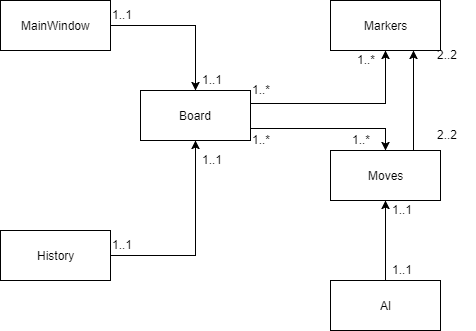
\includegraphics[scale = 0.4]{class-diagram}
  	\caption{Class Diagram- basic class diagram}
  	\label{fig:nonfloat}
	\end{figure}
To begin with six classes would be needed beginning with MainWindow.cs for the GUI, a Board class to build the board, a Marker Class to make each marker, an AI Class which would be implemented once a fully functional player vs player was completed, a History for storing games and a Move class to check for valid moves.This was later changed to incorporate extra features like the options menu and replay options window.

	\subsection{Board}
	\begin{figure}[H]
  	\centering
  	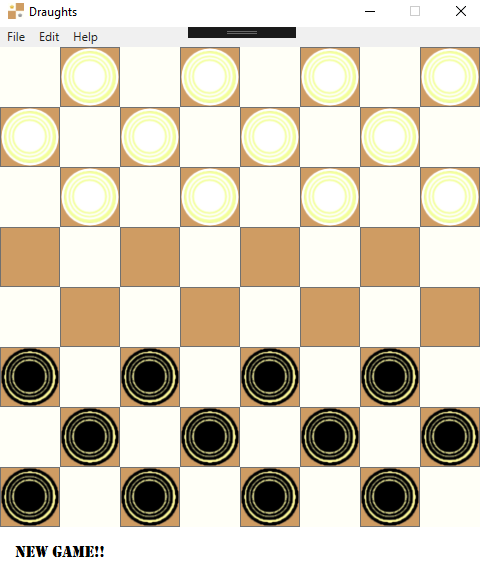
\includegraphics[scale = 0.4]{board}
  	\caption{Board and Markers - GUI of game board with markers ready to play}
  	\label{fig:nonfloat}
	\end{figure}

	To begin with the board was made using a 2D int array 8,8 so each square could be assigned to a number(-1 for invalid squares, 0 for empty squares, 1 White markers, 2 Black markers, 3 White kings, 4 Black kings) after the board was created in a text based environment and markers were placed using a the number system,it was at this point the decision to use a GUI would be a better representation for the game. The board was recreated in a GUI using stack-panels still with the same underlying numbering system. The empty board is created with buttons on the stack panels to allow the user to select them once marker are placed. The button is named with it row and column number.
	
	\subsection{Markers}
	The second stage of development moved on placing markers on the board a case statement was used to determine the placement of the markers, this is a more effective way to carryout the placement than the original way it was done in the text-based version which was a series of "if" statements. The markers are built using the Marker class which contains three values: the markers row and column and wither or not it has been promoted to a king. After placement is determined the marker gets added to the corresponding stack panel for that row and column, the button's name get updated with what the Marker colour is either black or white. An image of the marker is placed as the background of the button to show users what each button represents. Below is an image of the standard markers.
	\begin{figure}[H]
  	\centering
  	
\includegraphics[scale = 1.25]{Marker}
	\caption{Markers - game markers, White and Black Markers}
  	\label{fig:nonfloat}
	\end{figure}
	
	\subsection{Moves}
	The Move class  is used to create check move validation and checking if a jump move is available(take an opponents marker). Move validation is done by passing the marker colour to a method within the move class, It then checks to see if the placement chosen for the move is one column plus or minus one to the current column and plus a row for whites or minus a row for the blacks, this is done with four "if" statements. the other two check if the marker has a promotion and therefore can move up or down the rows regardless of colour.  If the move is invalid a message box appears telling the user that it is invalid with a reason as to why.
	\begin{figure}[H]
  	\centering
  	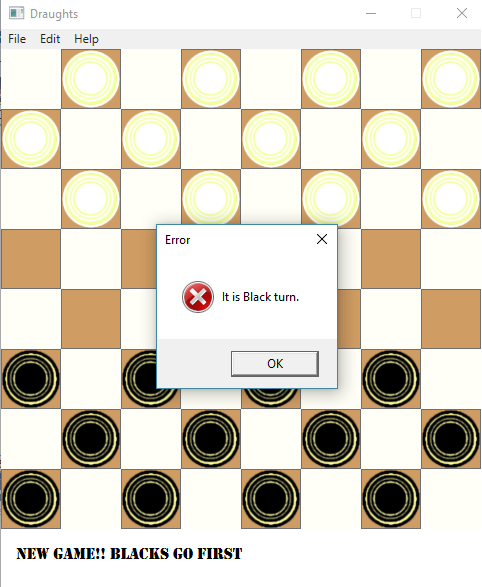
\includegraphics[scale = 0.5]{errors}
	\caption{Invalid move -message box showing error when moving a white marker of a black turn}
  	\label{fig:nonfloat}
	\end{figure}
	
	
Jumps validation is done using a series of if statements just like the move validation, but it checks two columns and plus or minus two rows depending on colour and promotion status. The jump possibilities get added to a list there if the list is populated a jump must occur.  
this is done by checking the number status on the board e.g On a "White" turn, a two indicting the that square is occupied by a "Black" marker it will then check if the square behind is a zero and that option will be added to the list of jumps. An "if" statement is the used if the list.Count() is greater than zero a jump must occur.  
Promotions are dealt with in the MainWindow.cs in a KingMe method. that uses two "if" statements one for if the marker is "white" and the row is equal to eight. (bottom of the board for whites) or marker equal "black" and row equal to zero (top of the board for the blacks). If a marker is to be promoted the button name gets updated with the appropriate king either "WhiteKing" or "BlackKing" and the button's background image gets updated with the appropriate king image.
\begin{figure}[H]
  	\centering
  	
\includegraphics[scale = 1.25]{KingMarkers}
	\caption{Markers - game markers for promotion, White and Black King-Markers}
  	\label{fig:nonfloat}
	\end{figure} 
	\subsection{Player vs Player}
	Player vs Player (PVP) was done first to allow the game's logic to be fully tested therefore eliminating invalid moves that a player could make and therefore an AI player would not be-able to make as well. Making the game PVP first then adding AI later, allowed future features such as an undo feature to be added without impacting the games logic.  The winning condition is calculated by counting each players markers. and if any of the counts return a zero the other player wins.
	
	\subsection{Undo/Redo}
	Once the PVP was fully working, the next stage was to get an undo feature working. To do this a stack was created so that when a player moves a marker.The undo feature is triggered by a player using the menu or by the standard MS Windows keyboard shortcut "CTRL + Z". The undo\_stack gets added to after every move, a stack was chosen as the data structure for this as the last move in has to be the first move back out a Deque was considered for this feature as it would double for the replay feature later on. however Deques are not natively supported by C\#. The undo is preformed play switches back to the other who's move was undo if multiple undos are preformed play will switch to the player who's move was undo last, e.g if "Black" player undoes two moves play would stay with the "Black" player if they done three moves play would return to "White" player. Originally the stack just held the position before and after into the stack in the order of the before row, before column, after row, after column. however after the redo feature was completed the stacked needed to also hold the promotion status of a marker. 
\\
The redo feature was built using a stack as well, this stack gets added to only after an undo move is made to allow a player to undo the undo automatically using the menu or the standard MS Windows keyboard shortcut "CTRL + Y".  It also became apparent that an extra stack would needed for both undo and redo features to store taken markers in order to return them to the board if a move redone after an undo had occurred.
	
	\subsection{AI}
The AI was developed using a variation of the Fisher-Yates Shuffle algorithm. In this algorithm it puts all possibilities into list and randomly eliminates options until only one remains, The AI class uses a variation of this in which each marker is checked to see if a zero is in an adjacent square, returned a zero indicates an empty square it will then add that possibility to a list of moves and then a random int taken from zero to list.Count() and make the move that matches the position within the list, however if it finds a two indicting the that square is occupied by a "Black" marker it will then check if the square behind is a zero and take the jump, since a jump is mandatory in draughts, the same as in a PVP game.

The AI method within MainWindow.cs is an asynchronous method, this is done to give the player a better chance to what marker the AI has moved and to give an illusion that the AI is thinking about a move. An asynchronous method had to be used instead of a standard thread.Sleep() as this would sleep the threat and not update the GUI until the very end and lock out the user.
Below is the segment of code that delays the AI the time is done in milliseconds and could be change to give a more instantaneous response.
\begin{lstlisting}[caption =code to delay the AI for 1 second]
 async Task PutTaskAIDelay()
        {
            await Task.Delay(1000);
        }
\end{lstlisting}
	
	\subsection{Game Replay}
The replay Game feature was the last feature to be added it was at this point additional classes were required these were a Singleton List class, a ReplayWindow.cs Class and a Replay class. to replay a  the games uses one queue and two stacks. 

A queue is used to store each of the moves just like the undo feature as mentioned above a deque was considered for the role. the queue allows for each move to be added one at a time by row,column,promotion status, also a first in first out which is required to show the flow of play.  

The two stacks being used are for taken markers like in the undo and redo feature however a temporary stack is needed to flip the stack around so the taken markers are popped out in the right order. The first stack is created in when the game board is cleared a copy of the retaken\_stack is copied into he replay taken stack.

The Singleton List pattern this was chosen as only one instance of a list to store previous games is required and a Singleton prevent multiple instances from being created by mistake however it does create a global variable which some may view as a bad practice.

The ReplayWindow.cs give the user a GUI to select which game to replay, with an option at what speed to play the game back at fast, medium or slow speed these done using a ComboBox, The replay comboBox is populated on the window opening and populated with gameids from the Singleton game list.
 \begin{figure}[H]
  	\centering
  	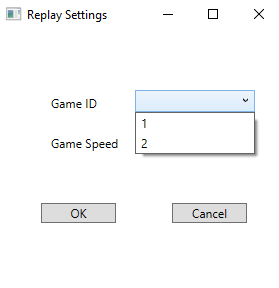
\includegraphics[scale = 0.5]{ReplayWindow}
	\caption{Replay - ReplayWindow.cs, User selection for game and speed of replay}
  	\label{fig:nonfloat}
	\end{figure}

The replay is an asynchronous method like the AI. this was done as with the move a happened instantaneously and showed only the final outcome so a async was added to let the user see where each marker moved to and in what order. The delay is set by default to  two second delay but can be changed in the replay option window to fast being one second, medium being two seconds and slow being five seconds.

The replay class is only executed hold a the game that is currently being replayed so it can be viewed again as when each turn is dequed from history it was originally lost.

	
	\section{Enhancements}
Extra features and functionality that was added in to enhance the user experience they have no real impact on how the game runs were as follows:

An Options window to change game settings.
\begin{figure}[H]
  	\centering
  	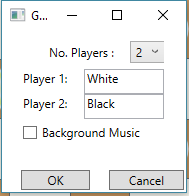
\includegraphics[scale = 0.5]{Options}
	\caption{Options - OptionsWindow.cs, Game settings show the default settings for games}
  	\label{fig:nonfloat}
	\end{figure}

Background Music, royalty free background music was added, as this is a personal choice for the user the music is by default turned off but can be turned on the options menu.

Player Names, To add a more personal touch to the game players change the names of the players, This is just a cosmetic effect and does not affect internal logic of turns. the only difference is in the bottom the label and error messages will display the players name instead of the "Black" or "White.
\begin{figure}[H]
  	\centering
  	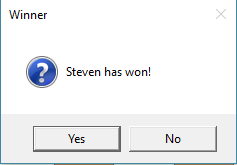
\includegraphics[scale = 0.75]{Winner}
	\caption{Personalisation  - Winner message,personalised Winner message}
  	\label{fig:nonfloat}
	\end{figure}

The game also has a help feature for users who are not familiar with how to draughts or checkers this is a message box with the game's rules and winning condition. This accesable via the help menu or the standard MS Windows keyboard shortcut "F1".
\begin{figure}[H]
  	\centering
  	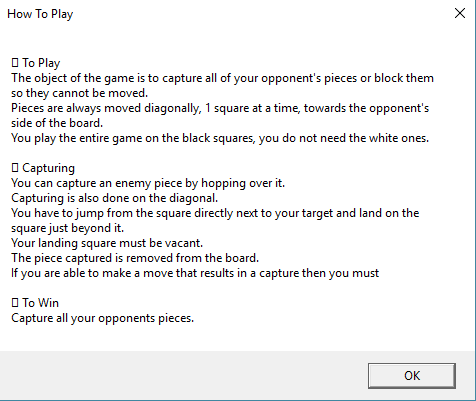
\includegraphics[scale = 0.75]{Help}
	\caption{Help Menu  - rules and wining condition for draughts}
  	\label{fig:nonfloat}
	\end{figure}

As stated above standard MS Windows keyboard he washortcuts where implemented through out the project. To give a more user friendly and professional product. 

Using the MoSCoW method of agile development, the following are extra features that would have been added are as follows:
AI vs AI

Persistence of Data
CSV not working cant store queues and stacks, futrue try storing in json

Custom Backgrounds 
more cosmetic dropped due to time restraint

	
	would like to have :AI VS AI, Game replays saved to a file for persistence
	
	\section{Critical Evaluation}
	x

	\section{Personal Evaluation}
	x
    
   
   


		
\end{document}